% Provenance (never printed): old terminale S material on mountain ranges and
% continental collision (folds, reverse faults and nappes as signs of
% shortening and thickening; ophiolites and sutures as the trace of a closed
% ocean; the Himalaya and the Alps as examples). Owner (Sync 0): collision,
% fold/anticline/syncline/fold axis, reverse fault/thrust, nappe, ophiolite,
% suture, shortening. Fault is Book 1's (g7), normal fault g11.05's, the root
% and Airy isostasy g11.03's and g12.01's: recalled, never redefined. India's
% past latitudes: figdata/grade-12/india_drift.py (GPlates Web Service, two
% published plate models); shortening: figdata/grade-12/fold_shortening.py;
% the belt map: figdata/grade-12/alpine_belt.py.
\chapter{Pembentukan Pegunungan}\label{ch:g12:mountain-building}

Para pendaki yang mencapai puncak Gunung Everest, \qty{8848.86}{m} di atas
permukaan laut, berdiri di atas batu kapur. Ahli geologi yang membawa turun
contoh-contoh batuan dari puncak itu menemukan di dalamnya pecahan-pecahan
trilobit, ostrakoda, dan krinoid: makhluk laut yang hidup lebih dari 440 juta
tahun yang lalu, pada zaman Ordovisium. Batuan tertinggi di dunia diendapkan di
dasar sebuah laut. Bab ini menjelaskan bagaimana dasar laut sampai ke atap
dunia: dua benua bertumbukan, dan kerak di antara keduanya terjepit, terlipat,
tertumpuk, dan menebal menjadi sebuah pegunungan.
% ledger: sakai05:summit, tulane:roots (marine limestones at the top of Mt. Everest), ics:base.Ordovician, ics:base.Silurian (486.85-443.1 Ma); Book 1: tht:everest (8848.86 m)

\begin{omfigure}
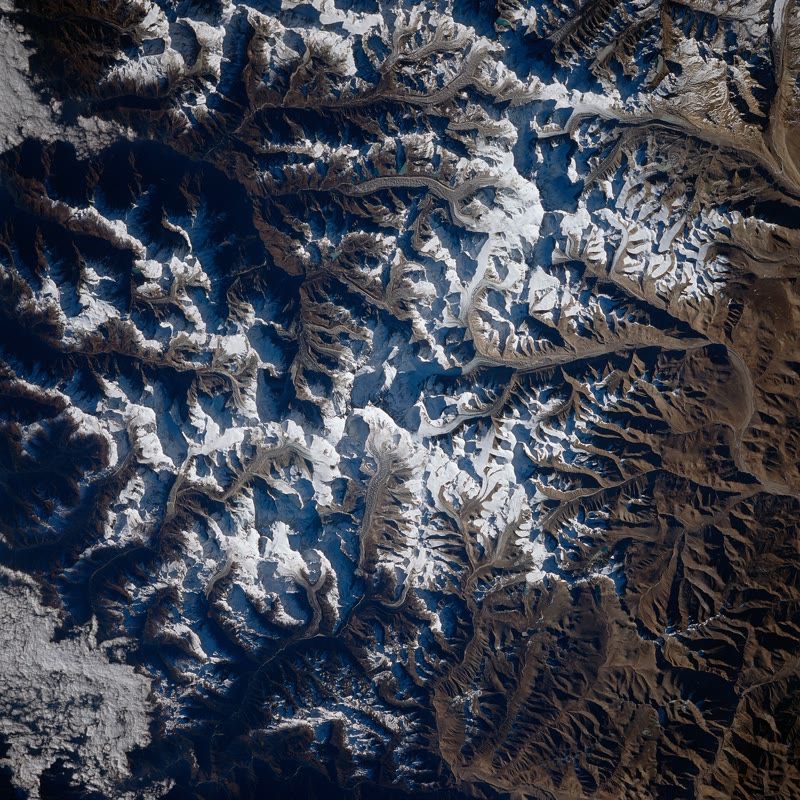
\includegraphics[width=0.5\linewidth]{images/book2/g12-nasa-everest-columbia.jpg}

{\small Gunung Everest dan banyak gletser di sekitarnya, dilihat dari pesawat
ulang-alik Columbia pada 30 November 1996. Foto NASA (domain publik).}
\end{omfigure}
% ledger: photo:g12-everest-columbia

\begin{recall}
Lempeng \omterm{def:g11:ocean-ridges:oceanic-lithosphere}{litosfer samudra}, yang dibuat di punggungan, tenggelam kembali ke dalam
mantel di palung; \omterm{def:g11:subduction-zones:slab}{lempengannya} menariknya ke bawah
(\cref{ch:g11:subduction-zones}). \omterm{def:g12:continental-crust:continental-crust}{Kerak benua} tebal dan ringan, rata-rata
sekitar \qty{2830}{kg/m^3} dibandingkan dengan \qty{3380}{kg/m^3} untuk mantel
di bawahnya, sehingga kerak itu mengapung tinggi, dan kerak yang tebal berdiri
lebih tinggi daripada kerak yang tipis, di atas sebuah \omterm{def:g12:continental-crust:root}{akar}
(\cref{ch:g12:continental-crust,ch:g11:lithosphere-asthenosphere}). Sesar
adalah rekahan yang di sepanjangnya kedua blok telah bergerak; pada \omterm{def:g11:ocean-ridges:normal-fault}{sesar
normal}, blok di atas bidang sesar telah bergerak turun, seperti di tempat kerak
teregang pada punggungan yang lambat (\cref{ch:g11:ocean-ridges}).
\end{recall}
% ledger: cm95:crust, data:prem, tulane:no-subduct, usgs:normal-fault

\section{Dari subduksi ke tumbukan}

Samudra yang dihabiskan di palung lebih cepat daripada dibuat di punggungannya
akan menyusut. Benua yang menumpang pada lempeng yang tenggelam makin mendekati
palung dengan kecepatan lempeng itu, dan akhirnya tiba di sana. \omterm{def:g11:ocean-ridges:oceanic-lithosphere}{Litosfer
samudra} di depannya telah turun; benua itu tidak dapat mengikutinya, karena
keraknya terlalu ringan untuk tenggelam ke dalam mantel yang lebih rapat.
\omterm{def:g11:subduction-zones:subduction}{Subduksi} berhenti. Kedua benua terjepit satu sama lain, dan \omterm{def:g11:subduction-zones:slab}{lempengan} yang
tergantung dari dasar samudra itu akhirnya patah lepas dan tenggelam ke dalam
mantel.
% ledger: earle:collision, tulane:no-subduct

\begin{definition}[Tumbukan benua]\label{def:g12:mountain-building:collision}
Yang disebut \emph{tumbukan benua}\index{tumbukan benua} adalah pertemuan dua
benua di batas lempeng konvergen, setelah \omterm{def:g11:ocean-ridges:oceanic-lithosphere}{litosfer samudra} di antara keduanya
tersubduksi. Tidak ada benua yang tenggelam: kerak di antara keduanya
terdeformasi dan menebal menjadi sebuah sabuk pegunungan.
\end{definition}
% ledger: earle:collision, tulane:no-subduct, usgs:himalaya-collision

\begin{omfigure}
\begin{tikzpicture}[x=0.95cm, y=0.95cm, font=\scriptsize]
  % ---- stage 1: the ocean closes ----
  \begin{scope}[yshift=0cm]
    \fill[omSea] (3.4,0) -- (8.6,0) -- (8.0,-0.5) -- (4.3,-0.5) -- (3.5,0.0) -- cycle;
    \fill[omLithGranite] (0,0.15) -- (3.5,0.15) -- (4.3,-0.5) -- (4.3,-0.75) -- (3.5,-1.0) -- (0,-1.0) -- cycle;
    \fill[omLithBasalt] (4.3,-0.5) -- (8.0,-0.5) .. controls (9.0,-0.75) and (9.6,-1.2) .. (10.4,-2.0)
      -- (10.15,-2.15) .. controls (9.4,-1.4) and (8.9,-1.0) .. (8.0,-0.75) -- (4.3,-0.75) -- cycle;
    \fill[omLithGranite] (8.0,-0.5) -- (8.6,0.2) -- (12,0.2) -- (12,-1.05) -- (9.5,-1.05)
      .. controls (9.0,-0.75) .. (8.0,-0.5) -- cycle;
    \fill[omThm!70] (10.0,0.2) -- (10.3,0.55) -- (10.6,0.2) -- cycle;
    \draw[black!60, line width=0.3pt] (0,0.15) -- (3.5,0.15) -- (4.3,-0.5) -- (8.0,-0.5) -- (8.6,0.2) -- (12,0.2);
    \draw[-{Stealth[length=2mm]}, line width=0.8pt] (1.2,0.45) -- (2.6,0.45);
    \node[anchor=east] at (0,-0.4) {1};
    \node at (1.8,-0.5) {benua};
    \node at (6.1,-0.25) {samudra};
    \node[anchor=north] at (6.1,-0.8) {litosfer samudra};
    \node[anchor=south] at (8.0,0.0) {palung};
    \node[anchor=south] at (10.3,0.55) {busur gunung api};
    \node at (11.1,-0.5) {benua};
  \end{scope}
  % ---- stage 2: the continents meet ----
  \begin{scope}[yshift=-3.0cm]
    \fill[omSea] (6.9,0) -- (8.4,0) -- (8.0,-0.4) -- (7.4,-0.35) -- cycle;
    \fill[omLithGranite] (0,0.15) -- (6.8,0.15) -- (7.6,-0.4) -- (8.0,-0.5)
      .. controls (9.0,-0.75) .. (9.5,-1.05) -- (9.2,-1.4) -- (6.5,-1.0) -- (0,-1.0) -- cycle;
    \fill[omLithBasalt] (9.5,-1.05) .. controls (10.0,-1.4) .. (10.6,-2.0) -- (10.35,-2.15)
      .. controls (9.8,-1.6) .. (9.2,-1.4) -- cycle;
    \fill[omLithGranite] (8.0,-0.5) -- (8.6,0.2) -- (12,0.2) -- (12,-1.05) -- (9.5,-1.05)
      .. controls (9.0,-0.75) .. (8.0,-0.5) -- cycle;
    \fill[omLithPeridotite] (7.0,0.15) -- (7.9,0.15) -- (8.3,0.05) -- (7.95,-0.12) -- (7.3,0.0) -- cycle;
    \fill[omThm!70] (10.0,0.2) -- (10.3,0.55) -- (10.6,0.2) -- cycle;
    \draw[-{Stealth[length=2mm]}, line width=0.8pt] (3.2,0.45) -- (4.6,0.45);
    \node[anchor=east] at (0,-0.4) {2};
    \node at (3.4,-0.45) {benua};
    \draw[black!60] (7.6,0.12) -- (7.0,0.75) node[anchor=south east, inner sep=1pt] {irisan dasar samudra};
    \node at (11.1,-0.5) {benua};
    \node[anchor=west] at (10.7,-1.9) {lempengan};
  \end{scope}
  % ---- stage 3: a mountain belt ----
  \begin{scope}[yshift=-6.4cm]
    \fill[omLithGranite] (0,0.15) -- (4.5,0.15) .. controls (6.0,0.4) and (6.6,1.25) .. (7.6,1.3)
      .. controls (8.7,1.3) and (9.6,0.5) .. (10.6,0.2) -- (12,0.2) -- (12,-1.05) -- (10.6,-1.1)
      .. controls (9.5,-2.2) and (8.6,-2.6) .. (7.7,-2.6) .. controls (6.6,-2.6) and (5.6,-1.6) .. (4.5,-1.0)
      -- (0,-1.0) -- cycle;
    \draw[black!60, line width=0.3pt] (0,0.15) -- (4.5,0.15) .. controls (6.0,0.4) and (6.6,1.25) .. (7.6,1.3)
      .. controls (8.7,1.3) and (9.6,0.5) .. (10.6,0.2) -- (12,0.2);
    \draw[black!60, dashed, line width=0.4pt] (0,-1.0) -- (4.5,-1.0) .. controls (5.6,-1.6) and (6.6,-2.6) .. (7.7,-2.6)
      .. controls (8.6,-2.6) and (9.5,-2.2) .. (10.6,-1.1) -- (12,-1.05);
    \draw[omThm, line width=1.0pt] (7.0,1.25) -- (8.3,-2.55);
    \foreach \t in {0.15,0.4,0.65}
      \fill[omLithPeridotite] ($(7.0,1.25)!\t!(8.3,-2.55)$) ++(-0.12,0.05) -- ++(0.3,0) -- ++(-0.05,-0.22) -- ++(-0.3,0) -- cycle;
    \fill[omLithBasalt] (10.9,-1.9) -- (11.5,-2.35) -- (11.35,-2.5) -- (10.75,-2.05) -- cycle;
    \node[anchor=east] at (0,-0.4) {3};
    \node at (2.4,-0.45) {benua};
    \node at (11.3,-0.5) {benua};
    \draw[black!60] (7.2,0.6) -- (5.9,1.5) node[anchor=east, inner sep=1pt] {sutura dengan ofiolit};
    \node at (7.7,-1.9) {akar};
    \node[anchor=north] at (11.2,-2.5) {lempengan yang patah lepas};
    \node[anchor=south] at (7.6,1.35) {sabuk pegunungan};
  \end{scope}
\end{tikzpicture}

{\small Dari \omterm{def:g11:subduction-zones:subduction}{subduksi} ke tumbukan (tidak berskala). 1: sebuah samudra menutup
ketika dasarnya tenggelam di palung. 2: benua tiba di palung dan tidak dapat
tenggelam; irisan-irisan dasar samudra terdorong ke atas tepinya. 3: kerak di
antara kedua benua memendek dan menebal menjadi sabuk pegunungan yang berdiri
di atas sebuah \omterm{def:g12:continental-crust:root}{akar}; garis tempat kedua benua bersatu, yang ditandai oleh
irisan-irisan dasar samudra, adalah \omterm{def:g12:mountain-building:suture}{sutura}; \omterm{def:g11:subduction-zones:slab}{lempengan} itu patah lepas dan
tenggelam.}
\end{omfigure}
% ledger: earle:collision, tulane:ocean-basins, usgs:suture, tulane:roots

\subsection{Jejak samudra yang lenyap}

Setelah samudra itu menutup, kedua benua terlas di sepanjang sebuah garis.

\begin{definition}[Sutura]\label{def:g12:mountain-building:suture}
Yang disebut \emph{sutura}\index{sutura} adalah garis, atau zona sempit, yang
di sepanjangnya dua benua telah disatukan oleh tumbukan, setelah \omterm{def:g11:subduction-zones:subduction}{subduksi} di
antara keduanya berhenti: jejak sebuah batas lempeng masa lalu. Sutura
menandai tempat samudra di antara keduanya dahulu berada.
\end{definition}
% ledger: usgs:suture, liu20:itsz

Apa yang menandai sebuah \omterm{def:g12:mountain-building:suture}{sutura}? Di sepanjang banyak \omterm{def:g12:mountain-building:suture}{sutura} terdapat tubuh-tubuh
batuan yang tidak termasuk di bagian mana pun dari sebuah benua: dari atas ke
bawah, sedimen laut, basalt bantal, sekumpulan \omterm{def:g11:igneous-rocks:intrusion}{retas} tegak yang berdiri
berdampingan, \omterm{def:g11:ocean-ridges:gabbro}{gabro}, dan di dasarnya \omterm{def:g11:ocean-ridges:peridotite}{peridotit} mantel: lapisan-lapisan dasar
samudra (\cref{ch:g11:ocean-ridges}), dengan bagian atas mantel di bawahnya.
% ledger: tulane:ocean-basins

\begin{definition}[Ofiolit]\label{def:g12:mountain-building:ophiolite}
Yang disebut \emph{ofiolit}\index{ofiolit} adalah sepotong \omterm{def:g11:ocean-ridges:oceanic-lithosphere}{litosfer samudra} ---
sedimen, basalt bantal, \omterm{def:g11:igneous-rocks:intrusion}{retas} berlapis, \omterm{def:g11:ocean-ridges:gabbro}{gabro}, dan \omterm{def:g11:ocean-ridges:peridotite}{peridotit} mantel --- yang
terdorong ke atas \omterm{def:g12:continental-crust:continental-crust}{kerak benua}.
\end{definition}
% ledger: tulane:ocean-basins

\omterm{def:g12:mountain-building:ophiolite}{Ofiolit} adalah dasar samudra yang terdampar: seiris samudra yang lenyap, yang
terdorong ke atas sebuah benua alih-alih tenggelam bersama bagian lainnya.
Pegunungan yang terangkat oleh tumbukan umumnya mengandung sebagian \omterm{def:g11:ocean-ridges:oceanic-lithosphere}{kerak
samudra} dan mantel atas, karena di situlah sebuah samudra menutup. Di Tibet
selatan, \omterm{def:g12:mountain-building:ophiolite}{ofiolit-ofiolit} yang berjajar di sepanjang \omterm{def:g12:mountain-building:suture}{sutura} Indus--Tsangpo
adalah sisa-sisa samudra yang disebut Neo-Tethys, yang dahulu terletak di
antara India dan wilayah Lhasa; sebuah \omterm{def:g11:ocean-ridges:gabbro}{gabro} di sana telah ditentukan umurnya
243 juta tahun.
% ledger: tulane:ocean-basins, earle:collision, liu20:itsz

\begin{omfigure}
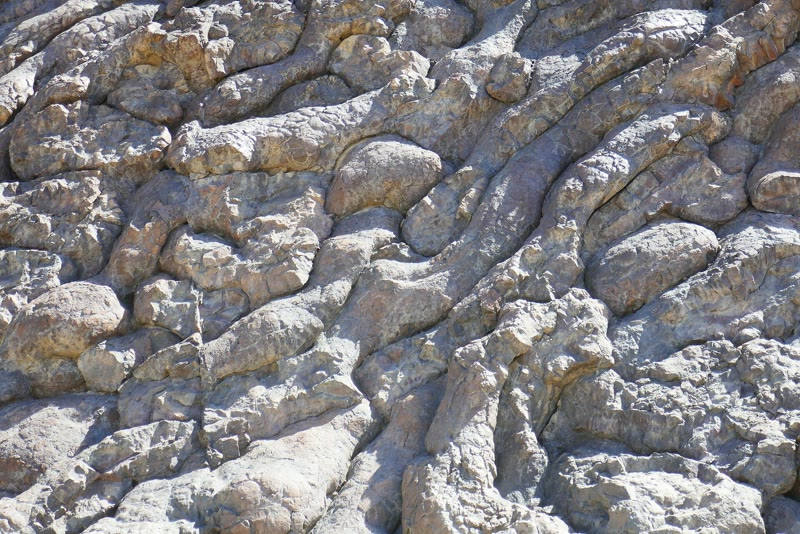
\includegraphics[width=0.6\linewidth]{images/book2/g12-duchoiselle-oman-pillows.jpg}

{\small Lava bantal \omterm{def:g12:mountain-building:ophiolite}{ofiolit} Semail di Wadi Jizzi, Oman: lava yang mendingin di
bawah air sebagai bantal-bantal yang membulat, kini berada di darat. Foto
Lionel Duchoiselle (CC~BY-SA~3.0).}
\end{omfigure}
% ledger: photo:g12-oman-pillows

\section{Memendekkan kerak}

Bila terjepit dari samping, tubuh batuan akan patah jika dingin dan getas; jika
cukup hangat untuk berperilaku plastis, tubuh batuan itu terlipat. Sabuk
pegunungan penuh dengan \omterm{def:g12:mountain-building:fold}{lipatan} maupun sesar.
% ledger: earle:folds

\subsection{Lipatan}

\begin{definition}[Lipatan; antiklin; sinklin; sumbu lipatan]\label{def:g12:mountain-building:fold}
Yang disebut \emph{lipatan}\index{lipatan} adalah lengkungan pada lapisan-lapisan
batuan. Sisi-sisinya yang miring adalah \emph{sayap}; sayap-sayap itu bertemu di
\emph{engsel}, tempat lapisan-lapisan paling melengkung, dan garis di sepanjang
engsel adalah \emph{sumbu lipatan}\index{sumbu lipatan}. Yang disebut
\emph{antiklin}\index{antiklin} adalah lipatan yang lapisan-lapisannya
melengkung ke atas, dengan sayap-sayap yang miring menjauhi sumbu; yang disebut
\emph{sinklin}\index{sinklin} adalah lipatan yang lapisan-lapisannya melengkung
ke bawah, dengan sayap-sayap yang miring menuju sumbu.
\end{definition}
% ledger: earle:folds, tulane:fold-geometry

Bidang yang melalui engsel-engsel lapisan yang berurutan adalah bidang sumbu.
\omterm{def:g12:mountain-building:fold}{Antiklin} dan \omterm{def:g12:mountain-building:fold}{sinklin} biasanya muncul berpasangan, dengan sayap yang satu
sekaligus menjadi sayap yang berikutnya. \omterm{def:g12:mountain-building:fold}{Lipatan} ada dalam segala ukuran, dari
yang mikroskopis sampai yang lebarnya puluhan kilometer. Setelah tererosi,
\omterm{def:g12:mountain-building:fold}{antiklin} memperlihatkan lapisan-lapisan tertuanya di intinya dan \omterm{def:g12:mountain-building:fold}{sinklin}
lapisan-lapisan termudanya; \omterm{def:g12:mountain-building:fold}{antiklin} belum tentu berupa punggung bukit, dan
\omterm{def:g12:mountain-building:fold}{sinklin} belum tentu berupa lembah, karena erosi mengikuti lapisan yang keras dan
yang lunak, bukan bentuk \omterm{def:g12:mountain-building:fold}{lipatannya}.
% ledger: earle:folds, tulane:fold-geometry

\begin{omfigure}
\begin{tikzpicture}[x=1.2cm, y=1.2cm, font=\scriptsize]
  \def\W{6}\def\H{2.0}\def\dx{1.35}\def\dy{0.78}
  \tikzset{declare function={zb(\x,\c)=\c+0.8*cos(60*(\x-1.5));}}
  \colorlet{bandA}{omLithSchist!70}\colorlet{bandB}{omLithSand}\colorlet{bandC}{omLithShale}
  \colorlet{bandD}{icsJurassic!35}\colorlet{bandE}{icsTriassic!35}\colorlet{bandF}{icsCretaceous!45}
  % front face
  \begin{scope}
    \clip (0,0) rectangle (\W,\H);
    \fill[bandA] (0,0) rectangle (\W,\H);
    \foreach \c/\col in {0.0/bandB, 0.6/bandC, 1.2/bandD, 1.8/bandE, 2.4/bandF}
      \fill[\col] plot[domain=0:\W, samples=80, smooth] (\x,{zb(\x,\c)}) -- (\W,4) -- (0,4) -- cycle;
    \foreach \c in {0.0,0.6,1.2,1.8,2.4}
      \draw[black!55, line width=0.35pt] plot[domain=0:\W, samples=80, smooth] (\x,{zb(\x,\c)});
  \end{scope}
  % top face: outcrop bands (crossings of the top surface computed for these curves)
  \fill[bandE] (0,\H) -- (0.242,\H) -- ++(\dx,\dy) -- (\dx,\H+\dy) -- cycle;
  \fill[bandD] (0.242,\H) -- (2.758,\H) -- ++(\dx,\dy) -- (0.242+\dx,\H+\dy) -- cycle;
  \fill[bandE] (2.758,\H) -- (3.5,\H) -- ++(\dx,\dy) -- (2.758+\dx,\H+\dy) -- cycle;
  \fill[bandF] (3.5,\H) -- (5.5,\H) -- ++(\dx,\dy) -- (3.5+\dx,\H+\dy) -- cycle;
  \fill[bandE] (5.5,\H) -- (\W,\H) -- ++(\dx,\dy) -- (5.5+\dx,\H+\dy) -- cycle;
  \foreach \x in {0.242,2.758,3.5,5.5} \draw[black!55, line width=0.35pt] (\x,\H) -- ++(\dx,\dy);
  % right face: the layers meet it at constant heights (cylindrical folds)
  \foreach \lo/\hi/\col in {0.0/0.6/bandB, 0.6/1.2/bandC, 1.2/1.8/bandD, 1.8/2.0/bandE}
    \fill[\col] (\W,\lo) -- (\W+\dx,\lo+\dy) -- (\W+\dx,\hi+\dy) -- (\W,\hi) -- cycle;
  \foreach \y in {0.6,1.2,1.8} \draw[black!55, line width=0.35pt] (\W,\y) -- ++(\dx,\dy);
  % outline
  \draw[black, line width=0.5pt] (0,0) rectangle (\W,\H) (0,\H) -- (\dx,\H+\dy) -- (\W+\dx,\H+\dy) -- (\W,\H)
    (\W+\dx,\H+\dy) -- (\W+\dx,\dy) -- (\W,0);
  % fold axes on the top face, axial planes on the front face
  \draw[omThm, line width=1pt] (1.5,\H) -- ++(\dx,\dy);
  \draw[omDef, line width=1pt] (4.5,\H) -- ++(\dx,\dy);
  \draw[omThm, dashed, line width=0.6pt] (1.5,0) -- (1.5,\H);
  \draw[omDef, dashed, line width=0.6pt] (4.5,0) -- (4.5,\H);
  \node[anchor=south, omThm] at (1.5+\dx,\H+\dy) {antiklin: sumbu lipatan};
  \node[anchor=south, omDef] at (4.5+\dx,\H+\dy) {sinklin: sumbu lipatan};
  \draw[black!70] (3.2,0.95) -- (3.9,-0.35) node[anchor=north] {sayap};
  \draw[black!70] (1.5,1.4) circle (0.07) -- (0.4,-0.35) node[anchor=north] {engsel};
  \draw[black!70] (1.5,0.25) -- (2.0,-0.35) node[anchor=north] {bidang sumbu};
\end{tikzpicture}

{\small Sebuah \omterm{def:g12:mountain-building:fold}{antiklin} dan sebuah \omterm{def:g12:mountain-building:fold}{sinklin}, yang terpotong oleh permukaan erosi
yang datar (diagram blok, tidak berskala). Sumbu-sumbu \omterm{def:g12:mountain-building:fold}{lipatan} berjalan di
sepanjang engsel; garis-garis putus-putus adalah jejak bidang-bidang sumbu. Di
permukaan atas, \omterm{def:g12:mountain-building:fold}{antiklin} yang tererosi memperlihatkan lapisan yang lebih tua di
intinya, \omterm{def:g12:mountain-building:fold}{sinklin} lapisan yang lebih muda.}
\end{omfigure}
% ledger: earle:folds, tulane:fold-geometry

\begin{omfigure}
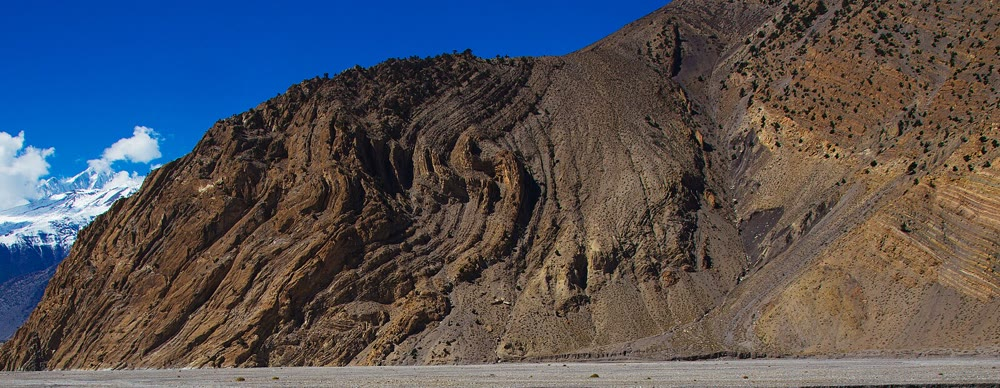
\includegraphics[width=0.95\linewidth]{images/book2/g12-hullot-kali-gandaki-folds.jpg}

{\small Lapisan-lapisan batuan yang terlipat pada sebuah tebing di Himalaya,
sekitar \qty{3}{km} di timur laut Jomsom di ngarai Kali Gandaki, Nepal. Foto
Jean-Marie Hullot (CC~BY~2.0).}
\end{omfigure}
% ledger: photo:g12-kali-gandaki

\omterm{def:g11:fossil-fuel-geology:reservoir}{Batuan penutup} Perbukitan Varden terlipat dengan cara yang sama, tetapi jauh
lebih landai. Batu pasir, batu kapur, serpih, dan kapurnya diendapkan mendatar,
lalu dilengkungkan menjadi sebuah \omterm{def:g12:mountain-building:fold}{antiklin} dan sebuah \omterm{def:g12:mountain-building:fold}{sinklin} yang
sayap-sayapnya miring \ang{12}; sebuah \omterm{def:g11:ocean-ridges:normal-fault}{sesar normal} yang lebih muda
memotongnya.
% ledger: region:name; model in figdata/shared/region.py (LIMB_DIP 12, AXIS_ANTI 3.5 km, AXIS_SYN 7.5 km)

\begin{omfigure}
\begin{tikzpicture}
\begin{axis}[omsection, x=1.25cm, y=0.003125cm, xmin=0, xmax=9.49, ymin=-700, ymax=650,
  xlabel={jarak dari A (\unit{km})}, ylabel={ketinggian (\unit{m})},
  ytick={-600,-300,0,300,600}, tick label style={font=\scriptsize}]
\addplot[fill=black!8, draw=black!50, line width=0.3pt, even odd rule] table {figdata/out/shared-region-section-unit-schist.dat};
\addplot[fill=icsTriassic!20, draw=black!50, line width=0.3pt, even odd rule] table {figdata/out/shared-region-section-unit-sandstone.dat};
\addplot[fill=icsJurassic!25, draw=black!50, line width=0.3pt, even odd rule] table {figdata/out/shared-region-section-unit-limestone.dat};
\addplot[fill=icsJurassic!8, draw=black!50, line width=0.3pt, even odd rule] table {figdata/out/shared-region-section-unit-shale.dat};
\addplot[fill=icsCretaceous!20, draw=black!50, line width=0.3pt, even odd rule] table {figdata/out/shared-region-section-unit-chalk.dat};
\addplot[fill=omLithAlluv, draw=black!50, line width=0.3pt, even odd rule] table {figdata/out/shared-region-section-unit-alluvium.dat};
\addplot[black, line width=0.7pt] table {figdata/out/shared-region-section-ground.dat};
\addplot[fault] table {figdata/out/shared-region-section-fault.dat};
% axis positions from figdata/grade-12/fold_shortening.py (section_anticline_km, section_syncline_km; the syncline lies on the hanging wall, shifted by the fault heave)
\draw[omThm, dashed, line width=0.7pt] (axis cs:3.162,-700) -- (axis cs:3.162,660);
\draw[omDef, dashed, line width=0.7pt] (axis cs:7.484,-700) -- (axis cs:7.484,660);
\node[anchor=south, omThm, font=\scriptsize] at (axis cs:3.162,660) {sumbu antiklin};
\node[anchor=south, omDef, font=\scriptsize] at (axis cs:7.484,660) {sumbu sinklin};
\node[anchor=south east, font=\small\bfseries] at (axis cs:0,650) {A};
\node[anchor=south west, font=\small\bfseries] at (axis cs:9.49,650) {B};
\node[font=\scriptsize, fill=white, inner sep=1pt] at (axis cs:1.2,-520) {sekis};
\node[font=\scriptsize, fill=white, inner sep=1pt, anchor=east] at (axis cs:6.55,-450) {sesar normal};
\end{axis}
\end{tikzpicture}

\smallskip
{\small\tikz\fill[black!8, draw=black!50] (0,0) rectangle (0.35,0.22);~sekis \quad
\tikz\fill[icsTriassic!20, draw=black!50] (0,0) rectangle (0.35,0.22);~batu pasir \quad
\tikz\fill[icsJurassic!25, draw=black!50] (0,0) rectangle (0.35,0.22);~batu kapur \quad
\tikz\fill[icsJurassic!8, draw=black!50] (0,0) rectangle (0.35,0.22);~serpih \quad
\tikz\fill[icsCretaceous!20, draw=black!50] (0,0) rectangle (0.35,0.22);~kapur \quad
\omve{2.5}}

{\small Penampang A--B melintasi Perbukitan Varden, dari barat daya ke timur
laut. \omterm{def:g11:fossil-fuel-geology:reservoir}{Batuan penutup} terletak di atas batuan dasar sekis dan terlipat menjadi
sebuah \omterm{def:g12:mountain-building:fold}{antiklin} dan sebuah \omterm{def:g12:mountain-building:fold}{sinklin}; \omterm{def:g11:ocean-ridges:normal-fault}{sesar normal}, yang lebih muda daripada
\omterm{def:g12:mountain-building:fold}{lipatan-lipatan} itu, menurunkan blok timur laut. Skala vertikalnya diregangkan
2.5 kali, sehingga sayap-sayapnya tampak lebih curam daripada kenyataannya.
Data: model wilayah dari seri buku ini.}
\end{omfigure}
% ledger: region:name; computed in figdata/shared/region.py (section A-B)

\subsection{Sesar naik, sesar anjak, dan nappe}

Di tempat kerak terjepit ketika masih dingin dan getas, kerak itu patah di
sepanjang sesar dari jenis yang berbeda dengan \omterm{def:g11:ocean-ridges:normal-fault}{sesar normal} pada kerak yang
teregang.

\begin{definition}[Sesar naik; sesar anjak]\label{def:g12:mountain-building:thrust}
Yang disebut \emph{sesar naik}\index{sesar naik} adalah sesar miring yang di
sepanjangnya blok di atas bidang sesar telah bergerak naik terhadap blok di
bawahnya. Sesar naik terbentuk di tempat kerak terjepit. Yang disebut
\emph{sesar anjak}\index{sesar anjak} adalah sesar naik dengan kemiringan
landai, kurang dari \ang{45}.
\end{definition}
% ledger: earle:reverse-thrust, tulane:fold-geometry

\omterm{def:g12:mountain-building:thrust}{Sesar anjak} dapat membawa selembar batuan sejauh puluhan kilometer, sehingga
batuan yang lebih tua akhirnya terletak di atas batuan yang lebih muda,
berlawanan dengan urutan pengendapannya. Di Pegunungan Rocky, Sesar Anjak
McConnell telah mendorong setumpuk batuan sedimen setebal sekitar
\qty{800}{m} sejauh kira-kira \qty{40}{km} dari barat ke timur: batu kapur yang
berumur sekitar 500 juta tahun kini terletak di atas batu lumpur yang berumur
sekitar 75 juta tahun.
% ledger: earle:reverse-thrust

\begin{definition}[Nappe]\label{def:g12:mountain-building:nappe}
Yang disebut \emph{nappe}\index{nappe} adalah lembaran batuan yang besar yang
telah terbawa jauh, sering kali puluhan kilometer, di atas batuan di bawahnya
di sepanjang \omterm{def:g12:mountain-building:thrust}{sesar anjak} yang hampir datar.
\end{definition}
% ledger: ngu:nappe, earle:reverse-thrust

\omterm{def:g12:mountain-building:nappe}{Nappe} dapat membawa batuan yang terbentuk jauh dari situ, bahkan irisan dasar
samudra; \omterm{def:g12:mountain-building:nappe}{nappe} itu sendiri dapat terlipat, dengan lapisan-lapisan yang
terbalik. Sabuk pegunungan menumpuk \omterm{def:g12:mountain-building:nappe}{nappe} yang satu di atas yang lain. Erosi
kemudian melubangi sebuah \omterm{def:g12:mountain-building:nappe}{nappe}, membuka jendela ke batuan di bawahnya, dan
meninggalkan kepingan-kepingan \omterm{def:g12:mountain-building:nappe}{nappe} yang terpisah di atas batuan yang lebih
muda.
% ledger: ngu:nappe

\begin{omfigure}
\begin{tikzpicture}[x=1.0cm, y=1.0cm, font=\scriptsize]
  % rocks in place (younger), flat-lying
  \fill[icsCretaceous!25] (0,-1.6) rectangle (12,-0.4);
  \fill[icsJurassic!25] (0,-1.6) rectangle (12,-1.1);
  \draw[black!50, line width=0.3pt] (0,-1.1) -- (12,-1.1);
  \fill[white] (5.6,-0.4) -- (6.2,-0.62) -- (6.8,-0.4) -- cycle;
  % the nappe (older rocks) above a nearly flat thrust, cut by erosion
  \fill[omLithSchist!80] (0.8,-0.4) .. controls (1.2,0.35) and (1.9,0.35) .. (2.3,-0.4) -- cycle;
  \fill[omLithSchist!80] (3.2,-0.4) .. controls (3.9,0.9) and (4.8,0.9) .. (5.6,-0.4) -- cycle;
  \fill[omLithSchist!80] (6.8,-0.4) .. controls (7.1,0.9) and (7.7,1.3) .. (8.4,1.25) -- (12,0.9) -- (12,-0.4) -- cycle;
  % ground surface
  \draw[black, line width=0.6pt] (0,-0.4) -- (0.8,-0.4) .. controls (1.2,0.35) and (1.9,0.35) .. (2.3,-0.4)
     -- (3.2,-0.4) .. controls (3.9,0.9) and (4.8,0.9) .. (5.6,-0.4) -- (6.2,-0.62) -- (6.8,-0.4)
     .. controls (7.1,0.9) and (7.7,1.3) .. (8.4,1.25) -- (12,0.9);
  % thrust traces (teeth on the block that moved over)
  \draw[thrust fault] (0.8,-0.4) -- (2.3,-0.4);
  \draw[thrust fault] (3.2,-0.4) -- (5.6,-0.4);
  \draw[thrust fault] (6.8,-0.4) -- (12,-0.4);
  \draw[-{Stealth[length=2mm]}, line width=0.9pt] (11.4,1.45) -- (9.6,1.6);
  \node[anchor=south] at (10.5,1.55) {gerak nappe};
  \node at (9.9,0.3) {nappe: batuan yang lebih tua};
  \node[fill=white, inner sep=1pt] at (2.0,-0.85) {batuan di tempat: lebih muda};
  \draw[black!60] (1.55,0.0) -- (1.3,0.8) node[anchor=south] {kepingan terpisah};
  \draw[black!60] (6.2,-0.58) -- (6.2,-0.68) node[anchor=north, fill=white, inner sep=1pt] {jendela};
  \draw[black!60] (9.0,-0.42) -- (9.3,-0.68) node[anchor=north, fill=white, inner sep=1pt] {sesar anjak};
\end{tikzpicture}

{\small Sebuah \omterm{def:g12:mountain-building:nappe}{nappe} (tidak berskala): lembaran batuan yang lebih tua yang
terbawa di sepanjang \omterm{def:g12:mountain-building:thrust}{sesar anjak} yang hampir datar di atas batuan yang lebih
muda yang tetap di tempatnya. Erosi telah memotong sebuah jendela menembusnya
dan meninggalkan sekeping darinya yang terpisah di sebelah kiri. Gigi-gigi pada
\omterm{def:g12:mountain-building:thrust}{sesar anjak} menunjuk ke arah blok yang bergerak naik di atasnya.}
\end{omfigure}
% ledger: ngu:nappe, earle:reverse-thrust

\begin{omfigure}
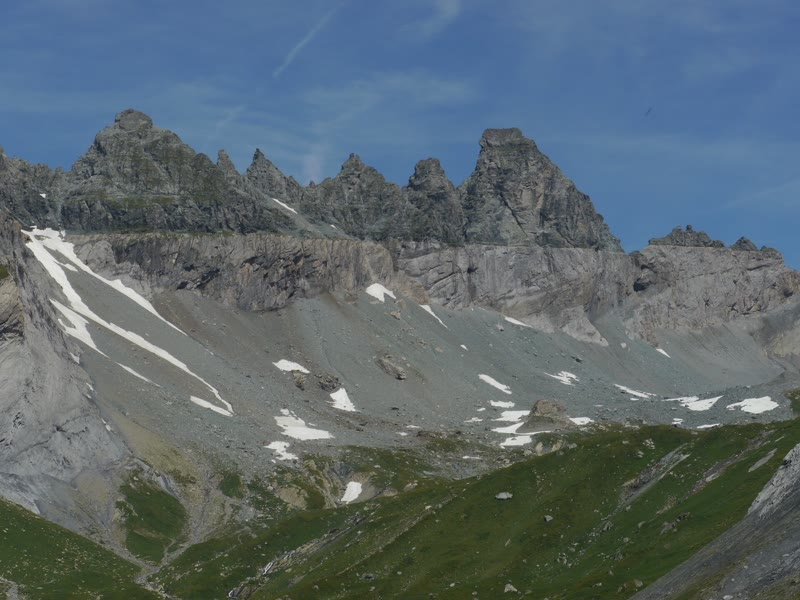
\includegraphics[width=0.5\linewidth]{images/book2/g12-heine-glarus-thrust.jpg}

{\small Sesar Anjak Glarus di Pegunungan Alpen di Swiss timur. Batuan gelap di
puncak-puncaknya, yang diendapkan pada zaman Perm, antara sekitar 299 dan 252
juta tahun yang lalu, terletak di atas batuan yang lebih terang dan jauh lebih
muda; \omterm{def:g12:mountain-building:thrust}{sesar anjak} itu adalah batas tajam di antara keduanya. Batuan bagian atas
telah berpindah sekitar 40 sampai \qty{50}{km}. Foto Christian Heine
(CC~BY-SA~3.0).}
\end{omfigure}
% ledger: photo:g12-glarus (Verrucano, Permian; displacement 40-50 km, Pfiffner 1985), ics:base.Permian, ics:base.Triassic

\subsection{Mengukur pemendekan}

\omterm{def:g12:mountain-building:fold}{Lipatan} dan \omterm{def:g12:mountain-building:thrust}{sesar anjak} sama-sama membuat kerak lebih pendek ke arah kerak itu
terjepit.

\begin{definition}[Pemendekan]\label{def:g12:mountain-building:shortening}
Yang disebut \emph{pemendekan}\index{pemendekan} sebuah lapisan adalah fraksi
panjangnya yang telah hilang: bila panjangnya semula $L_0$ dan kini
membentang sejauh $L$,
\[
  e = \frac{L_0 - L}{L_0}.
\]
\end{definition}

Untuk mengukurnya, diperlukan panjang semula $L_0$. Pada banyak \omterm{def:g12:mountain-building:fold}{lipatan},
lapisan-lapisannya mempertahankan tebalnya ketika melengkung, saling menggeser
seperti halaman-halaman buku yang dibengkokkan; lapisan seperti itu tidak
teregang di sepanjang panjangnya. Hal ini memberikan panjang semulanya.
% ledger: tulane:fold-geometry (flexural folds keep their thickness)

\begin{proposition}[Pemendekan lapisan yang terlipat]\label{prop:g12:mountain-building:shortening}
Bila sebuah lapisan terlipat tanpa teregang atau terjepit di sepanjang dirinya,
panjang semulanya $L_0$ adalah panjangnya yang diukur di sepanjang lapisan yang
terlipat itu. Untuk \omterm{def:g12:mountain-building:fold}{lipatan} dengan sayap lurus yang miring dengan sudut
$\theta$,
\[
  e = 1 - \cos\theta .
\]
\end{proposition}

\begin{proof}
Bila lapisan itu dibuka \omterm{def:g12:mountain-building:fold}{lipatannya}, tanpa diregangkan, lapisan itu terbentang
datar dengan panjang yang tidak berubah; jadi $L_0$ adalah panjang di sepanjang
lapisan. Pada sayap lurus sepanjang $\ell$ yang miring dengan sudut $\theta$,
jarak mendatar yang ditempuh adalah $\ell\cos\theta$ (segitiga siku-siku).
Dengan menjumlahkan semua sayap, lapisan yang panjangnya $L_0$ membentang sejauh
$L = L_0\cos\theta$, dan $e = (L_0 - L_0\cos\theta)/L_0 =
1 - \cos\theta$.
\end{proof}

\begin{omfigure}
\begin{tikzpicture}
\begin{axis}[name=sine, x=2.0cm, y=2.0cm, axis lines=none,
  xmin=-0.05, xmax=2.25, ymin=-0.4, ymax=0.8, clip=false]
% computed in figdata/grade-12/fold_shortening.py (part sine: A/lambda = 0.25, e = 31.7 %)
\addplot[omLithSand!80!black, line width=1.6pt] table[x=x, y=y] {figdata/out/grade-12-fold_shortening-sine.dat};
\draw[omThm, line width=1.6pt] (axis cs:0,0.62) -- (axis cs:2.196,0.62);
\draw[black!60, |-|] (axis cs:0,-0.32) -- node[below, font=\scriptsize] {$L$ (kini)} (axis cs:1.5,-0.32);
\node[anchor=south west, font=\scriptsize, omThm] at (axis cs:0,0.64) {$L_0$: lapisan yang sama setelah dibuka lipatannya};
\end{axis}
\begin{axis}[omrecord, at={(sine.east)}, anchor=west, xshift=1.4cm, width=0.46\linewidth, height=4.6cm,
  xmin=0, xmax=80, ymin=0, ymax=85, xlabel={kemiringan sayap $\theta$ (\unit{\degree})},
  ylabel={pemendekan $e$ (\unit{\percent})}, xtick={0,20,...,80}]
% computed in figdata/grade-12/fold_shortening.py (part dip: e = 1 - cos theta)
\addplot[omProp, line width=1pt] table[x=theta, y=e_pct] {figdata/out/grade-12-fold_shortening-dip.dat};
\addplot[only marks, mark=*, mark size=1.6pt, omThm] coordinates {(12,2.185) (30,13.397) (60,50)};
\node[anchor=south, font=\scriptsize, align=center] at (axis cs:12,6) {Varden:\\\qty{2.2}{\percent}};
\node[anchor=west, font=\scriptsize] at (axis cs:32,10) {\qty{13}{\percent}};
\node[anchor=south east, font=\scriptsize] at (axis cs:60,51) {\qty{50}{\percent}};
\end{axis}
\end{tikzpicture}

{\small Kiri: sebuah lapisan yang terlipat membentang sejauh $L$; bila
dibentangkan datar, tanpa diregangkan, panjangnya $L_0$ (di sini tinggi \omterm{def:g12:mountain-building:fold}{lipatan}
seperempat panjang gelombangnya, dan $L$ adalah \qty{68}{\percent} dari $L_0$).
Kanan: \omterm{def:g12:mountain-building:shortening}{pemendekan} \omterm{def:g12:mountain-building:fold}{lipatan} dengan sayap lurus, $1 - \cos\theta$, terhadap
kemiringan sayapnya. \omterm{def:g12:mountain-building:fold}{Lipatan} yang landai hanya sedikit memendekkan lapisan.}
\end{omfigure}
% values: sine_025_e_pct 31.68 (L/L0 = 0.683); varden_e_pct 2.1852; chevron_30 13.397; chevron_60 50 (fold_shortening.py)

\begin{method}[Mengukur pemendekan pada penampang]\label{met:g12:mountain-building:shortening}
\begin{enumerate}
  \item Periksa bahwa penampang itu digambar menurut skala yang sebenarnya.
        Bila skala vertikalnya diregangkan, kemiringan dan panjang di sepanjang
        lapisan menjadi terlalu besar: gambarlah ulang, atau koreksi dahulu
        setiap kemiringan.
  \item Pilih satu batas lapisan yang dapat diikuti melintasi penampang;
        di tempat sebuah sesar memotongnya, sambungkan kedua ujung yang
        terpotong seperti keadaannya sebelum sesar itu bergerak.
  \item Ukur panjangnya di sepanjang lapisan, $L_0$: ikuti dengan seutas
        benang, atau jumlahkan potongan-potongan lurus yang pendek.
  \item Ukur jarak mendatar antara kedua ujungnya, $L$.
  \item Hitung $e = (L_0 - L)/L_0$; untuk sayap lurus yang kemiringannya
        diketahui, $e = 1 - \cos\theta$ langsung memberikannya.
\end{enumerate}
\end{method}

\begin{example}[Lipatan-lipatan Varden]\label{ex:g12:mountain-building:varden}
Sayap-sayap \omterm{def:g12:mountain-building:fold}{lipatan} Varden miring \ang{12}, sehingga \omterm{def:g11:fossil-fuel-geology:reservoir}{batuan penutupnya} memendek
sebesar $e = 1 - \cos\ang{12} = 1 - 0.978 = 0.022$, sekitar \qty{2.2}{\percent}:
sebuah jalur wilayah itu yang kini selebar \qty{10}{km} dahulu selebar $10/\cos\ang{12} \approx
\qty{10.22}{km}$ sebelum terlipat. Bila diukur pada penampang A--B seperti yang
digambar, sayap-sayap itu akan tampak miring sekitar \ang{28}, karena skala
vertikalnya diregangkan 2.5 kali: $\tan\theta$ dikalikan 2.5, dan $\arctan(2.5
\tan\ang{12}) \approx \ang{28}$. Bila dibaca apa adanya, hal itu akan
memberikan \omterm{def:g12:mountain-building:shortening}{pemendekan} \qty{12}{\percent}, lebih dari lima kali terlalu besar.
\end{example}
% values: varden_e_pct 2.1852, varden_L0_for_10km 10.223 (fold_shortening.py); arctan(2.5 x 0.2126) = 27.98 deg; 1 - cos 27.98 = 0.117

\omterm{def:g12:mountain-building:fold}{Lipatan} yang landai hanya menyerap sedikit. Sabuk yang terlipat ketat, dengan
sayap-sayap yang miring \ang{60}, telah memendek setengahnya; dan satu \omterm{def:g12:mountain-building:thrust}{sesar
anjak} yang hampir datar yang telah membawa sebuah \omterm{def:g12:mountain-building:nappe}{nappe} sejauh \qty{40}{km}
menyerap \omterm{def:g12:mountain-building:shortening}{pemendekan} \qty{40}{km}, sama banyaknya dengan sabuk \omterm{def:g12:mountain-building:fold}{lipatan} landai
yang sangat lebar.

\section{Penebalan dan pengangkatan}

\omterm{def:g12:mountain-building:shortening}{Pemendekan} tidak menghancurkan batuan. Sejalur kerak yang terjepit sampai
sebagian kecil dari lebarnya semula mempertahankan volumenya, sehingga kerak itu
pasti menebal: bila kerak setebal
$H_0$ dipendekkan dari lebar $L_0$ menjadi $L$ di sepanjang seluruh panjang
sabuk, penampangnya mempertahankan luasnya, $H L = H_0 L_0$, dan
\[
  H = H_0\,\frac{L_0}{L} = \frac{H_0}{1 - e}.
\]
Kerak setebal \qty{35}{km} yang memendek \qty{50}{\percent} menjadi setebal
\qty{70}{km}. Lalu \omterm{def:g11:lithosphere-asthenosphere:isostasy}{isostasi} melakukan sisanya: kerak yang lebih tebal mengapung
lebih tinggi, di atas \omterm{def:g12:continental-crust:root}{akar} yang lebih dalam (\cref{prop:g11:lithosphere-asthenosphere:airy}).
Dengan model Airy dan massa jenis dalam ingatan di atas, kerak yang lebih tebal
sebesar $\Delta H$ berdiri lebih tinggi sebesar $\Delta H\,(\rho_m - \rho_c)/\rho_m = \Delta H
\times 550/3380$, sekitar seperenam dari tebal tambahannya; lima perenam
sisanya membentuk \omterm{def:g12:continental-crust:root}{akar}. Kerak setebal \num{35} sampai \qty{40}{km} jauh dari
sabuk pegunungan, dan 50 sampai \qty{70}{km} di bawahnya: makin tinggi
pegunungan, makin tebal keraknya.
% ledger: tulane:roots, cm95:crust, data:prem

Beginilah batu kapur dasar laut sampai ke puncak Everest: diendapkan di dasar
sebuah laut, batu kapur itu terbawa ke utara bersama India, tertumpuk dalam
lembaran-lembaran \omterm{def:g12:mountain-building:thrust}{sesar anjak} Himalaya, dan terangkat ketika kerak di bawahnya
menebal dan naik. Gerak vertikal kerak seperti itu disebut pengangkatan.
% ledger: sakai05:summit, sakai05:stacking, tulane:roots (uplift), usgs:himalaya-collision

\section{Dua pegunungan}

\subsection{Himalaya}

Himalaya membentang \qty{2900}{km} di sepanjang perbatasan antara India dan
Tibet. Sekitar 80 juta tahun yang lalu India terletak kira-kira \qty{6400}{km}
di selatan Asia, di seberang sebuah samudra, dan bergerak ke utara dengan laju
sekitar \qty{9}{cm} setahun; India bertemu Asia antara 40 dan 50 juta tahun
yang lalu, dan gerak majunya ke utara kemudian melambat. Rekonstruksi lempeng
memperlihatkan perjalanan itu secara terperinci: disusun dari banyak jenis
bukti, di antaranya \omterm{def:g11:plate-motions:hotspot-track}{jejak titik panas} (\cref{ch:g11:plate-motions}),
rekonstruksi itu menggerakkan lempeng-lempeng mundur dalam waktu selangkah demi
selangkah.
% ledger: usgs:himalaya-collision, muller19:frame, muller22:frame

\begin{omfigure}
\begin{tikzpicture}
\begin{axis}[omrecord, omage, name=lat, width=0.5\linewidth, height=5.2cm,
  xmin=0, xmax=100, ymin=-45, ymax=35, xlabel={umur (\unit{Ma})}, ylabel={lintang (\unit{\degree})},
  xtick={0,20,...,100}, ytick={-40,-20,...,40},
  legend style={font=\scriptsize, at={(0.98,0.03)}, anchor=south east, fill=white}]
% computed in figdata/grade-12/india_drift.py (part lat; GPlates Web Service, MULLER2022 and MULLER2019)
\fill[omThm!12] (axis cs:40,-45) rectangle (axis cs:50,35);
\addplot[omThm, line width=1.1pt] table[x=age, y=m22_india] {figdata/out/grade-12-india_drift-lat.dat};
\addplot[omThm, dashed, line width=0.8pt] table[x=age, y=m19_india] {figdata/out/grade-12-india_drift-lat.dat};
\addplot[omDef, line width=1.1pt] table[x=age, y=m22_lhasa] {figdata/out/grade-12-india_drift-lat.dat};
\addplot[black!50, line width=0.4pt, forget plot] coordinates {(0,0) (100,0)};
\legend{{India tengah (2022)}, {India tengah (2019)}, {Lhasa (2022)}}
\end{axis}
\begin{axis}[omrecord, omage, at={(lat.east)}, anchor=west, xshift=1.9cm, width=0.42\linewidth, height=5.2cm,
  xmin=0, xmax=100, ymin=0, ymax=160, xlabel={umur (\unit{Ma})},
  ylabel={kecepatan ke utara (\unit{mm/yr})}, xtick={0,20,...,100}]
% computed in figdata/grade-12/india_drift.py (part steps: 5-Myr steps)
\fill[omThm!12] (axis cs:40,0) rectangle (axis cs:50,160);
\addplot[omThm, line width=1pt] table[x=age, y=m22] {figdata/out/grade-12-india_drift-steps.dat};
\addplot[omThm, dashed, line width=0.7pt] table[x=age, y=m19] {figdata/out/grade-12-india_drift-steps.dat};
\end{axis}
\end{tikzpicture}

{\small Kiri: lintang sebuah titik di India tengah (\ang{78}~BT,
\ang{20}~LU saat ini) dan Lhasa, di utara \omterm{def:g12:mountain-building:suture}{sutura}, selama 100 juta tahun
terakhir, dalam dua rekonstruksi lempeng yang telah diterbitkan (2022 dan
2019). Kanan: kecepatan India ke utara pada setiap langkah 5 juta tahun. Pita
yang diarsir menandai 40 sampai 50 juta tahun yang lalu. Data: R.~D.~Müller
dan kawan-kawan (2019, 2022), dihitung dengan GPlates Web Service.}
\end{omfigure}
% ledger: data:b2-gws-india, muller22:frame, muller19:frame; values: speed_65_50 128.5, speed_40_0 40.06, fastest 145.8 (50-55 Ma) (india_drift.py)

Kedua rekonstruksi itu sepakat sampai selisih beberapa derajat. Antara 65 dan
50 juta tahun yang lalu India bergerak ke utara dengan laju sekitar
\qty{13}{cm} setahun; antara 50 dan 40 juta tahun yang lalu kecepatannya
turun, dan
sejak 40 juta tahun yang lalu India bergerak dengan laju sekitar \qty{4}{cm}
setahun, kurang dari sepertiga kecepatan semula. Lhasa, di sisi Asia, juga
bergerak ke utara, tetapi jauh lebih lambat.
% values: speed_65_50 128.5 mm/yr, speed_40_0 40.06 mm/yr, slowdown_ratio 0.312 (india_drift.py)

\begin{example}[Kecepatan India]\label{ex:g12:mountain-building:india}
Dalam rekonstruksi tahun 2022, India tengah berada pada \ang{12.10}~LS 60 juta
tahun yang lalu dan pada \ang{0.68}~LS 50 juta tahun yang lalu. Satu derajat
lintang adalah
$2\pi R/360 = 2\pi \times \qty{6371}{km}/360 \approx \qty{111.2}{km}$. India
bergerak ke utara sejauh $(12.10 - 0.68) \times 111.2 \approx \qty{1270}{km}$
dalam 10 juta tahun: \qty{127}{km} per sejuta tahun, yaitu $\qty{127e6}{mm} /
\num{e6}\text{ tahun} = \qty{127}{mm}$, sekitar \qty{13}{cm}, setahun.
\end{example}
% ledger: data:b2-gws-india, earth:Rmean; values: lat 60 Ma -12.0964, 50 Ma -0.6801 (india_drift-lat)

Perlambatan itu dibaca sebagai tanda tumbukan: \omterm{def:g12:continental-crust:continental-crust}{kerak benua} yang tiba di palung
tidak dapat tenggelam, dan India tertahan. Tanggal persis kontak pertamanya
masih diperdebatkan: perkiraannya berkisar dari sekitar 60 sampai 54 juta tahun
yang lalu, dan sebagian ahli geologi berpendapat bahwa India mula-mula bertemu
dengan serangkaian pulau gunung api dan baru mencapai Asia sendiri sekitar 34
juta tahun yang lalu. India belum berhenti: kutub-kutub rotasi lempeng masa
kini menggerakkannya menuju Eurasia dengan laju sekitar \qty{4.5}{cm} setahun
melintasi Himalaya (\cref{ch:g11:plate-motions}), dan tekanannya menjepit
sebagian Asia ke arah timur.
% ledger: usgs:himalaya-collision, najman21:collision-age; values: today_in_eu_speed 44.99 mm/yr (india_drift.py, from nnr56:poles)

Di utara Himalaya, Dataran Tinggi Tibet rata-rata setinggi sekitar
\qty{4600}{m}, di atas kerak setebal sekitar \qty{70}{km}
(\cref{ch:g11:lithosphere-asthenosphere}). Di antara India dan Tibet terdapat
\omterm{def:g12:mountain-building:suture}{sutura} Indus--Tsangpo dengan \omterm{def:g12:mountain-building:ophiolite}{ofiolit-ofiolitnya}; di selatannya, Himalaya
sebagian besar tersusun dari sedimen yang diendapkan di tepi utara India, lalu
tertumpuk, terlipat, dan tersesarkan, termasuk batu kapur puncak Everest.
% ledger: karplus:tibet-moho, liu20:itsz, sakai05:stacking, sakai05:summit; Book 1: usgs:himalaya (Tibetan Plateau about 4600 m)

\subsection{Pegunungan Alpen, dan seluruh sabuknya}

Pegunungan Alpen mempunyai sejarah yang serupa dalam skala yang lebih kecil:
pegunungan itu terangkat di tempat Afrika bertumbukan dengan Eropa. Pegunungan
itu juga mengandung \omterm{def:g12:mountain-building:ophiolite}{ofiolit}, dan sesar-sesar anjak yang besar: pada Sesar
Anjak Glarus, batuan zaman Perm telah terbawa ke atas batuan yang jauh lebih
muda. Pegunungan Alpen dan Himalaya termasuk dalam satu sabuk pegunungan yang
panjang, melalui Zagros di Iran, tempat Afrika dan India bertumbukan dengan
Eurasia.
% ledger: earle:collision, photo:g12-glarus

\begin{omfigure}
\begin{tikzpicture}
\begin{axis}[axis equal image, xmin=-12, xmax=105, ymin=18, ymax=52, width=\linewidth,
  tick label style={font=\scriptsize}, xtick={0,30,60,90}, ytick={20,30,40,50},
  xticklabel={$\pgfmathprintnumber{\tick}^\circ$}, yticklabel={$\pgfmathprintnumber{\tick}^\circ$},
  axis background/.style={fill=omSea}, legend columns=3,
  legend style={font=\scriptsize, at={(0.5,-0.12)}, anchor=north, /tikz/every even column/.append style={column sep=5pt}}]
\addplot[fill=omLithAlluv, draw=black!45, line width=0.2pt, forget plot] table {figdata/out/shared-geo-land.dat};
% computed in figdata/grade-12/alpine_belt.py; ledger: data:etopo1, data:usgs-comcat
\addplot[only marks, mark=square*, mark size=1.15pt, omLithSand!85!black] table[x=lon, y=lat] {figdata/out/grade-12-alpine_belt-high.dat};
\addplot[only marks, mark=square*, mark size=1.15pt, omThm!75!black] table[x=lon, y=lat] {figdata/out/grade-12-alpine_belt-higher.dat};
\addplot[only marks, mark=*, mark size=0.7pt, black] table[x=lon, y=lat] {figdata/out/grade-12-alpine_belt-quakes.dat};
\addplot[omDef, line width=0.9pt, forget plot] table {figdata/out/shared-geo-school-collision.dat};
\addplot[black!70, line width=0.5pt, forget plot] table {figdata/out/shared-geo-school-subduction.dat};
\legend{{lebih tinggi dari \qty{1500}{m}}, {lebih tinggi dari \qty{3500}{m}}, {gempa bumi, magnitudo 6 atau lebih}}
\coordinate (alps) at (axis cs:9,48);
\coordinate (zagros) at (axis cs:46,23.5);
\coordinate (zagrosbelt) at (axis cs:50.5,31.5);
\coordinate (himal) at (axis cs:84,24);
\coordinate (tibet) at (axis cs:88,33);
\coordinate (arrA) at (axis cs:77,19.5);
\coordinate (arrB) at (axis cs:79.2,25);
\end{axis}
% labels drawn after the axis, so that no earthquake dot covers them
\node[font=\scriptsize, fill=white, inner sep=1pt, anchor=south] at (alps) {Alpen};
\draw[black!60, line width=0.4pt] (zagros) -- (zagrosbelt);
\node[font=\scriptsize, fill=white, inner sep=1pt] at (zagros) {Zagros};
\node[font=\scriptsize, fill=white, inner sep=1pt, anchor=west] at (himal) {Himalaya};
\node[font=\scriptsize, fill=white, inner sep=1pt] at (tibet) {Dataran Tinggi Tibet};
\draw[-{Stealth[length=2mm]}, line width=1pt, omProp] (arrA) -- (arrB);
\end{tikzpicture}

{\small Sabuk pegunungan muda dari Atlantik sampai Tibet: daerah tinggi (setiap
persegi adalah sel 1 derajat), gempa bumi dangkal bermagnitudo 6 atau lebih
dari tahun 1976 sampai 2025 (lebih dangkal dari \qty{70}{km}), dan batas-batas
tumbukan antarlempeng (garis biru). Panah menunjukkan gerak India menuju
Eurasia. Data: ETOPO1, katalog gempa bumi USGS, batas lempeng dari Bird (2003),
daratan dari Natural Earth.}
\end{omfigure}
% ledger: data:etopo1, data:usgs-comcat, data:pb2002, data:ne-land; values: n_quakes 398 (alpine_belt.py)

Daerah tinggi dan gempa bumi mengikuti pita sempit yang sama. Tumbukan itu
belum selesai: gempa-gempa bumi menunjukkan bahwa kerak masih terus patah di
sepanjang seluruh sabuk, dan bahwa pegunungan masih terus terbentuk.

\section{Latihan}

\begin{exercise}[$\star$]\label{exo:g12:mountain-building:1}
Pasangkan setiap istilah dengan perinciannya: \omterm{def:g12:mountain-building:fold}{antiklin}, \omterm{def:g12:mountain-building:fold}{sinklin}, \omterm{def:g12:mountain-building:thrust}{sesar anjak},
\omterm{def:g12:mountain-building:nappe}{nappe}, \omterm{def:g12:mountain-building:suture}{sutura}, \omterm{def:g12:mountain-building:ophiolite}{ofiolit}. (a) \omterm{def:g12:mountain-building:thrust}{sesar naik} dengan kemiringan landai; (b) sepotong
dasar samudra yang ditemukan di darat; (c) \omterm{def:g12:mountain-building:fold}{lipatan} yang sayap-sayapnya miring
menuju sumbunya; (d) garis tempat dua benua bersatu; (e) \omterm{def:g12:mountain-building:fold}{lipatan} yang
sayap-sayapnya miring menjauhi sumbunya; (f) lembaran batuan yang besar yang
terbawa jauh di sepanjang \omterm{def:g12:mountain-building:thrust}{sesar anjak}.
\end{exercise}

\begin{exercise}[$\star$]\label{exo:g12:mountain-building:2}
Di seberang sebuah lembah, lapisan-lapisan di sisi barat miring \ang{20} ke
barat dan lapisan-lapisan di sisi timur miring \ang{20} ke timur. (1) Apakah
\omterm{def:g12:mountain-building:fold}{lipatan} di antara keduanya \omterm{def:g12:mountain-building:fold}{antiklin} atau \omterm{def:g12:mountain-building:fold}{sinklin}? (2) Setelah erosi, apakah
lapisan tertua atau termuda yang dijumpai di sepanjang sumbunya? (3) Apakah
lembah itu harus terletak di atas sebuah \omterm{def:g12:mountain-building:fold}{sinklin}?
\end{exercise}

\begin{exercise}[$\star$]\label{exo:g12:mountain-building:3}
Sebuah lapisan terlipat dengan sayap-sayap lurus yang miring \ang{30}.
(1) Hitung \omterm{def:g12:mountain-building:shortening}{pemendekannya}. (2) Kini lapisan itu membentang \qty{6.0}{km}. Berapa
panjangnya semula?
\end{exercise}

\begin{exercise}[$\star$]\label{exo:g12:mountain-building:4}
(1) Di sepanjang sebuah sesar, blok di atas bidang sesar telah bergerak turun.
Apakah sesar itu \omterm{def:g11:ocean-ridges:normal-fault}{sesar normal} atau \omterm{def:g12:mountain-building:thrust}{sesar naik}, dan apakah kerak itu teregang
atau terjepit? (2) Sebuah \omterm{def:g12:mountain-building:thrust}{sesar naik} miring \ang{25}: apakah sesar itu \omterm{def:g12:mountain-building:thrust}{sesar
anjak}?
\end{exercise}

\begin{exercise}[$\star$]\label{exo:g12:mountain-building:5}
(1) Urutkan batuan-batuan \omterm{def:g12:mountain-building:ophiolite}{ofiolit} ini dari atas ke bawah: \omterm{def:g11:ocean-ridges:gabbro}{gabro}, sedimen laut,
\omterm{def:g11:ocean-ridges:peridotite}{peridotit}, basalt bantal, \omterm{def:g11:igneous-rocks:intrusion}{retas} berlapis. (2) Mengapa basalt bantal
menunjukkan bahwa batuan itu terbentuk di bawah air? (3) Mengapa \omterm{def:g12:mountain-building:ophiolite}{ofiolit}
dijumpai di sepanjang \omterm{def:g12:mountain-building:suture}{sutura}?
\end{exercise}

\begin{exercise}[$\star\star$]\label{exo:g12:mountain-building:6}
Pada penampang berskala sebenarnya, sebuah batas batu pasir diikuti melalui
empat potongan lurus yang panjangnya \qty{2.1}{km}, \qty{1.8}{km},
\qty{2.4}{km}, dan \qty{1.6}{km}; kedua ujungnya berjarak \qty{6.0}{km}.
(1) Hitung \omterm{def:g12:mountain-building:shortening}{pemendekannya}. (2) Bila keempat sayap itu miring dengan sudut yang
sama, berapa sudutnya?
\end{exercise}

\begin{exercise}[$\star\star$]\label{exo:g12:mountain-building:7}
Blok atas sebuah \omterm{def:g12:mountain-building:thrust}{sesar anjak} yang miring \ang{10} telah bergerak \qty{45}{km}
di sepanjang bidang sesar. (1) Seberapa jauh blok itu bergerak mendatar?
(2) Seberapa tinggi blok itu naik? (3) Selebar apa sabuk \omterm{def:g12:mountain-building:fold}{lipatan} dengan
sayap-sayap yang miring \ang{12} yang akan menyerap \omterm{def:g12:mountain-building:shortening}{pemendekan} mendatar yang
sama?
\end{exercise}

\begin{exercise}[$\star\star$]\label{exo:g12:mountain-building:8}
Di sepanjang Sesar Anjak McConnell, batu kapur yang berumur sekitar 500 juta
tahun terletak di atas batu lumpur yang berumur sekitar 75 juta tahun.
(1) Prinsip penentuan umur relatif mana yang akan menyesatkan ahli geologi
yang mengabaikan sesar itu? (2) Berapa tahun lebih tua batuan bagian atas?
(3) Lembaran \omterm{def:g12:mountain-building:thrust}{sesar anjak} itu setebal sekitar \qty{800}{m} dan berpindah
\qty{40}{km}: berapa kali tebalnya sendiri jarak itu?
\end{exercise}

\begin{exercise}[$\star\star$]\label{exo:g12:mountain-building:9}
Dalam rekonstruksi tahun 2022, India tengah berada pada \ang{30.23}~LS 80 juta
tahun yang lalu dan pada \ang{19.38}~LS 66 juta tahun yang lalu. (1) Seberapa
jauh India bergerak ke utara? (2) Dengan kecepatan rata-rata berapa, dalam
\unit{cm} setahun? (3) Bandingkan dengan ringkasan dari US Geological Survey,
sekitar \qty{9}{m} seabad.
\end{exercise}

\begin{exercise}[$\star\star$]\label{exo:g12:mountain-building:10}
Kerak setebal \qty{35}{km} memendek \qty{40}{\percent} di sepanjang seluruh
sebuah sabuk. (1) Berapa tebalnya kemudian? (2) Dengan $\rho_c =
\qty{2830}{kg/m^3}$ dan $\rho_m = \qty{3380}{kg/m^3}$, seberapa lebih tinggi
kerak itu berdiri, dan seberapa dalam \omterm{def:g12:continental-crust:root}{akar} tambahannya?
\end{exercise}

\begin{exercise}[$\star\star$]\label{exo:g12:mountain-building:11}
Pada penampang yang skala vertikalnya diregangkan 3 kali, sebuah sayap tampak
miring \ang{40}. (1) Berapa kemiringan sebenarnya? (2) Hitung \omterm{def:g12:mountain-building:shortening}{pemendekan} dari
kemiringan sebenarnya dan dari kemiringan yang dibaca pada gambar. (3) Mengapa
penampang yang dipakai untuk mengukur \omterm{def:g12:mountain-building:shortening}{pemendekan} harus digambar menurut skala
yang sebenarnya?
\end{exercise}

\begin{exercise}[$\star\star\star$]\label{exo:g12:mountain-building:12}
\omterm{def:g12:mountain-building:fold}{Lipatan-lipatan} membulat yang digambar dalam bab ini, yang tingginya seperempat
panjang gelombangnya, mempunyai \omterm{def:g12:mountain-building:shortening}{pemendekan} \qty{31.7}{\percent}; kemiringan
tercuramnya sekitar \ang{57.5}. (1) Sebuah lapisan yang terlipat dengan cara ini
membentang \qty{10}{km}: berapa panjangnya semula? (2) Hitung \omterm{def:g12:mountain-building:shortening}{pemendekan}
\omterm{def:g12:mountain-building:fold}{lipatan} dengan sayap-sayap lurus pada \ang{57.5}. (3) Jelaskan mengapa \omterm{def:g12:mountain-building:fold}{lipatan}
bersayap lurus memendek lebih banyak untuk kemiringan tercuram yang sama.
\end{exercise}

\begin{exercise}[$\star\star\star$]\label{exo:g12:mountain-building:13}
Di utara Himalaya, pada \ang{85}~BT \ang{28}~LU, kutub-kutub rotasi memberi
India kecepatan terhadap Eurasia sebesar \qty{16.6}{mm/yr} ke timur dan
\qty{41.8}{mm/yr} ke utara. Selama 5 juta tahun terakhir, rekonstruksi tahun
2022 memberi India tengah kecepatan ke utara yang \qty{23.5}{mm/yr} lebih
besar daripada kecepatan Lhasa. (1) Tentukan kecepatan India terhadap Eurasia.
(2) Dengan menganggap komponen-komponen ke utara itu dapat dibandingkan,
berapa \omterm{def:g12:mountain-building:shortening}{pemendekan} utara--selatan per sejuta tahun yang tersisa untuk wilayah
di utara Lhasa? (3) Di bagian mana dalam bab ini terdapat tanda bahwa wilayah
ini sedang terdeformasi?
\end{exercise}

\begin{exercise}[$\star\star\star$]\label{exo:g12:mountain-building:14}
Di Pegunungan Alpen, sebuah \omterm{def:g12:mountain-building:nappe}{nappe} telah terbawa \qty{45}{km} di sepanjang
\omterm{def:g12:mountain-building:thrust}{sesar anjak} yang kemiringannya hampir nol. (1) Berapa \omterm{def:g12:mountain-building:shortening}{pemendekan} yang diserap
\omterm{def:g12:mountain-building:thrust}{sesar anjak} itu? (2) Berapa lebar, sebelum terlipat, \omterm{def:g11:fossil-fuel-geology:reservoir}{batuan penutup} yang
terlipat seperti di Perbukitan Varden (sayap \ang{12}) yang akan menyerap
\omterm{def:g12:mountain-building:shortening}{pemendekan} yang sama? (3) Apa yang ditunjukkan hal ini tentang cara sabuk
pegunungan menyerap konvergensi yang besar?
\end{exercise}

\begin{exercise}[$\star\star\star$]\label{exo:g12:mountain-building:15}
Batu kapur puncak Everest diendapkan di dasar laut, setidaknya sedikit di bawah
permukaan laut, dan kini berada pada ketinggian \qty{8848.86}{m}. (1) Dengan
menganggap tumbukan dimulai 50 juta tahun yang lalu, berapa laju pengangkatan
rata-rata yang terkecil, dalam \unit{mm} setahun? (2) Bandingkan dengan
kecepatan India sejak 40 juta tahun yang lalu, sekitar \qty{40}{mm} setahun.
(3) Mengapa pengangkatan batuan itu kemungkinan lebih besar daripada
ketinggiannya sekarang?
\end{exercise}

\begin{problem}[{Soal akhir pekan --- perjalanan India}]
\label{pb:g12:mountain-building:1}
% ledger: data:b2-gws-india, earth:Rmean, usgs:himalaya-collision, tulane:roots, cm95:crust, data:prem, karplus:tibet-moho; Book 1: usgs:himalaya (4600 m)
% values: india_drift-lat (MULLER2022, rounded to 0.01 deg); north_since_66_km 4378.7; converge_since_50 1354; gap_0 1073
Tabel berikut memberikan lintang sebuah titik di India tengah dan Lhasa, di
utara \omterm{def:g12:mountain-building:suture}{sutura}, dalam rekonstruksi lempeng tahun 2022 (negatif = selatan).
Ambillah satu derajat lintang sama dengan \qty{111.2}{km}, dan \qty{1}{km} per
sejuta tahun sama dengan \qty{1}{mm} setahun.

\begin{center}
\small
\begin{tabular}{|l|c|c|c|c|c|c|c|c|c|}
\hline
umur (\unit{Ma}) & 80 & 66 & 60 & 55 & 50 & 45 & 40 & 20 & 0 \\ \hline
India (\unit{\degree}) & $-30.23$ & $-19.38$ & $-12.10$ & $-7.24$ & $-0.68$ & 3.30 & 5.59 & 13.40 & 20.00 \\ \hline
Lhasa (\unit{\degree}) & & 19.48 & & & 21.15 & & & & 29.65 \\ \hline
\end{tabular}
\end{center}

\medskip
\noindent\textbf{Bagian I --- Lintang dan kecepatan.}
\begin{enumerate}
  \item Periksa nilai \qty{111.2}{km} untuk satu derajat, dengan $R =
        \qty{6371}{km}$.
  \item Kapan India tengah melintasi khatulistiwa?
  \item Seberapa jauh India bergerak ke utara dari 66 sampai 50 juta tahun
        yang lalu?
  \item Dengan kecepatan rata-rata berapa?
  \item Hitung kecepatannya pada setiap langkah dari 66 sampai 40 juta tahun
        yang lalu (66 sampai 60, 60 sampai 55, dan seterusnya). Pada langkah
        mana India paling cepat?
\end{enumerate}

\medskip
\noindent\textbf{Bagian II --- Perlambatan.}
\begin{enumerate}[resume]
  \item Hitung kecepatan rata-rata India dari 40 juta tahun yang lalu sampai
        kini.
  \item Berapa bagian dari kecepatannya dari 66 sampai 50 juta tahun yang lalu
        nilai itu?
  \item Di antara dua waktu manakah dalam tabel kecepatannya paling banyak
        turun?
  \item Mengapa tumbukan memperlambat lempeng?
  \item Seberapa jauh India bergerak ke utara dari 50 juta tahun yang lalu
        sampai kini?
\end{enumerate}

\medskip
\noindent\textbf{Bagian III --- Konvergensi yang terserap.}
\begin{enumerate}[resume]
  \item Seberapa jauh Lhasa bergerak ke utara dari 50 juta tahun yang lalu
        sampai kini?
  \item Seberapa banyak jarak utara--selatan antara India tengah dan Lhasa
        telah menyusut sejak 50 juta tahun yang lalu?
  \item Berapa jarak itu kini, dan berapa jarak itu 50 juta tahun yang lalu?
  \item Misalkan seluruh konvergensi ini diserap oleh \omterm{def:g12:mountain-building:shortening}{pemendekan} kerak di
        antara kedua titik itu. Berapa \omterm{def:g12:mountain-building:shortening}{pemendekan} $e$?
  \item Sebutkan dua jenis struktur yang menyerap \omterm{def:g12:mountain-building:shortening}{pemendekan} seperti itu.
\end{enumerate}

\medskip
\noindent\textbf{Bagian IV --- Kerak yang menebal.}
\begin{enumerate}[resume]
  \item Bila kerak itu setebal \qty{35}{km} 50 juta tahun yang lalu, berapa
        tebalnya sekarang, dengan mempertahankan luas penampangnya?
  \item Dengan $\rho_c = \qty{2830}{kg/m^3}$ dan $\rho_m = \qty{3380}{kg/m^3}$,
        seberapa tinggi kerak itu akan berdiri di atas arasnya semula?
  \item Dataran Tinggi Tibet setinggi sekitar \qty{4600}{m}, di atas kerak
        setebal sekitar \qty{70}{km}. Tebal kerak berapa yang diberikan model
        Airy untuk \qty{4600}{m}?
  \item Berikan satu alasan mengapa model sederhana pada pertanyaan 16
        melebih-lebihkan penebalan itu.
  \item Dengan menjumlahkan jarak pada pertanyaan 3 dan 10, seberapa jauh India
        telah berpindah ke utara sejak akhir zaman Kapur, 66 juta tahun yang
        lalu?
\end{enumerate}
\end{problem}
